\documentclass[a4paper, 12pt]{report}
    \parindent=1em
    \usepackage[font=footnotesize, labelfont=bf]{caption}  % bold caption
    %\usepackage[usenames,dvipsnames]{color}  % not compatible with knitr yet..
    \usepackage{xcolor}  % highlighting.
    \usepackage{enumerate}
    \usepackage{graphicx}  % rotate text
    \usepackage{listings}  % fancyvrb doesn't have word wrap..
        \lstset{
            basicstyle=\small\ttfamily,
            columns=flexible,
            breaklines=true,
            captionpos=t,  % sets the caption-position to bottom
            numbers=left,  % line numbers on the left
            frame=single,  % adds a frame around the code
            fontadjust=true
            escapechar=|
            language=HTML
        }
    \usepackage{url}
    \usepackage{tikz}
      \usetikzlibrary{decorations.text, arrows}  % decoration for for curved text
      \usetikzlibrary{positioning}  % for positioning nodes
    \usepackage{hyperref}
    \usetikzlibrary{shapes.geometric, arrows}
    \usepackage[export]{adjustbox}  % better image alignment & scale
    \usepackage{titlesec}  % chapter
        \titleformat
        {\chapter} % command
        [display] % shape
        {\bfseries\Large\itshape} % format
        {} % label
        {-15ex} % sep
        {
            \rule{\textwidth}{1pt}
            \vspace{1ex}
            \centering
        } % before-code
        [
        \vspace{-2ex}%
        \rule{\textwidth}{0.3pt}
        ] % after-code

%%%%% flow chart configuration %%%%%
\tikzstyle{simple} = [rectangle, rounded corners, text width=3cm, text centered, font=\small, draw=black, align=center, fill=green!20]
\tikzstyle{startstop} = [rectangle, rounded corners, minimum width=3cm, minimum height=1cm, text centered, draw=black, fill=green!20, font=\small]
\tikzstyle{process} = [rectangle, minimum width=2cm, minimum height=1cm, text centered, text width=1cm, draw=black, font=\small]
\tikzstyle{decision} = [diamond, minimum width=2cm, minimum height=1cm, text centered, draw=black, fill=green!30, font=\small]
\tikzstyle{arrow} = [thick,->,>=stealth]
\tikzstyle{line} = [thick,-,>=stealth]

\title{\textbf{Invertible Reproducible Documents}}
\author{Eric Lim}
\date{\today}

%\renewcommand\thesection{\arabic{section}}  % remove chapter numbering in section

\begin{document}
  \maketitle


%------------------------------------------------------------------------------
%------------------------------------------------------------------------------
%---------------------------- Chapter: Motivation -----------------------------
%------------------------------------------------------------------------------
%------------------------------------------------------------------------------
\chapter{Motivation}
\label{ch:motiv}

%<<setup, echo=FALSE>>=
%opts_chunk$set(comment = NA, prompt = TRUE, tidy = FALSE, background='white')
%options(prompt = "R> ")
%knit_theme$set("print")
%@

\textbf{Knitr(REF)} is a wonderful package that enables dynamic report generation with R. It allows integration of R code into LaTeX, LyX, HTML, Markdown, AsciiDoc, and reStructuredText documents through the concepts of literate programming (REF), which involves interaction between code and documentation for report generation. The main purpose of \textbf{knitr} follows an important idea in academic research that the ideal research paper or report must encompass the entire computational environment used to produce the results in the paper such as the code so that the same results can be reproduced using the same computational environment (reproducible research REF). The importance of reproducibility can be further extended to be applied in the entire area of academia (REF). %Reproducible Research: the Bottom Line by Jan de Leeuw

\begin{figure}[h]
\centering
  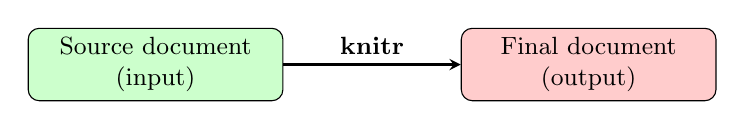
\begin{tikzpicture}[node distance=3cm]
    \node(in)[simple]{Source document \\ (input)};
    \node(out)[simple, fill=red!20, right of=in, xshift=2.5cm]{Final document \\ (output)};
    \draw[arrow](in)--node[anchor=south]{\small{\textbf{knitr}}} (out);
  \end{tikzpicture}
  \caption{Unidirectional document generation by \textbf{knitr}}
  \label{fig:1}
\end{figure}

While there are tremendously important ideas to consider and many advantages, the process of generating R code embedded documents using \textbf{knitr} is almost always a one-way trip (Figure \ref{fig:1}), meaning source documents (as input) can only generate final documents (as output), not the other way around. This is simply due to the fact that \textbf{knitr} is designed with intention to dynamically generate reports, not to extract displayed R code in final documents in order to generate source documents.

Consider a situation where a \emph{consultant} provides reports as reproducible documents and a \emph{client} is to read or review the reports. In this situation, it is often difficult for the consultant to receive feedback from the client efficiently. Since it is impossible to convert back from final documents to source documents, the client would have to provide his or her feedback by either writing physically on the printed copy of the final report or by electronic means such as through exchanging e-mails. The document provider, then, has to rectify the source documents accordingly, only to repeat the process of generating and presenting the report to the client. This process often has to be repeated until final correction can be achieved. As we can see, it can quickly become tedious.

We believe this is relevant to the field of statistics as similar situations mentioned above can often arise. Interaction between clients and consultants is crucial for statisticians and any possible factor to deteriorate the relationship with clients is best avoided. Therefore, we want to avoid this issue by a more efficient document generation workflow.

A possible solution is to allow clients to interact directly with the final documents and edit them. Then consultants can merge the changes and make final adjustments to generate new reports efficiently. In order to achieve this, reports must be \emph{invertible}, as well as reproducible, that is, final reports must be able to be converted into the source document format without introducing any change from the inversion process itself.

\begin{figure}[h]
\centering
  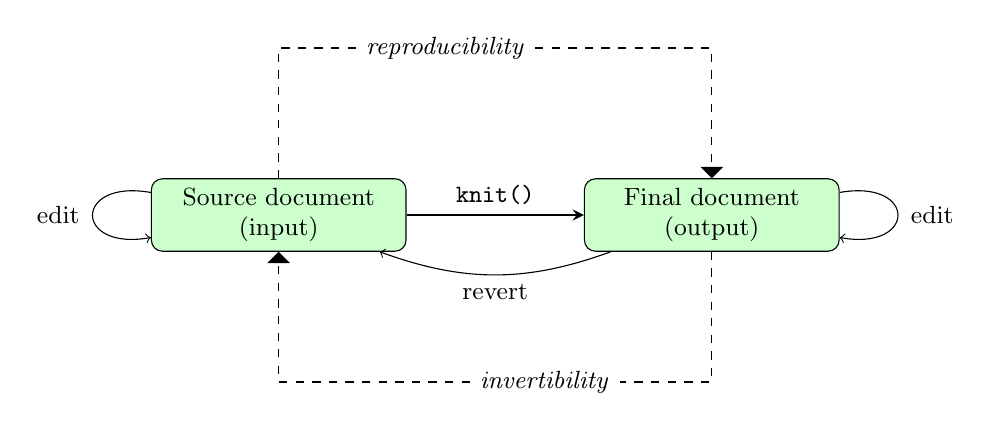
\begin{tikzpicture}[node distance=3cm]
    \node(in)[simple]{Source document \\ (input)};
    \node(out)[simple, right of=in, xshift=2.5cm] {Final document \\ (output)};
    \draw [arrow] (in)--node[anchor=south]{\small{\texttt{knit()}}} (out);
    \draw [->] (out) to [bend left=20] node[anchor=north] {\small{revert}} (in);
    \draw [->] (in) to [loop left, in=190, out=170, distance=1cm] (in) node[anchor=north, left of=in, xshift=2mm] {\small{edit}};
    \draw [->] (out) to [loop right, in=350, out=10, distance=1cm] (out) node[anchor=west, right of=out, xshift=-2mm] {\small{edit}};
    %
    \node(re) [above right of=in] {\small{\emph{reproducibility}}};
    \node(inv) [below left of=out] {\small{\emph{invertibility}}};
    \draw [dashed] (in)|-(re);
    \draw [dashed, arrows={-triangle 90}] (re)-|(out);
    \draw [dashed] (out)|-(inv);
    \draw [dashed, arrows={-triangle 90}] (inv)-|(in);
    %
    %\def\myshift#1{\raisebox{1ex}}  % so the text doesn't touch the line of arrow
    %\draw [dashed, ->, postaction={decorate, decoration={text along path, text align=center, text={|\small\myshift|reproducibility}}}] (in) to [bend left=60]  (out);
    %\def\myshift#1{\raisebox{-2.5ex}}
    %\draw [dashed, ->, postaction={decorate, decoration={text along path, text align=center, text={|\small\myshift|invertibility}}}] (out) to [bend left=60] (in);
    
    %\draw [dashed, ->] (in) to [bend left=60] node[anchor=north] {reproducibility} (out);
    %\draw [dashed, ->] (out) to [bend left=60] node[anchor=south] {invertibility} (in);
  \end{tikzpicture}
  \caption{Invertible reproducible workflow}
  \label{fig:2}
\end{figure}

This report introduces a possible workflow that can be utilised effectively in the aforementioned situation. The main focus of the project is in achieving this hypothetical round trip and exploring possible issues associated with it. Generalising the workflow by improving the robustness and efficiency of the functions involved has only been considered to a level that has been manageble under the time given for the project. Hence, it has been possible to devise two separate strategies to deal \emph{specifically} with two different document types under the allowed time. The phase 1 of this report will discuss primarily on dealing with HTML-based documents and the second phase will focus on Markdown-based documents.



%------------------------------------------------------------------------------
%------------------------------------------------------------------------------
%------------------------------ Chapter: R HTML -------------------------------
%------------------------------------------------------------------------------
%------------------------------------------------------------------------------
\chapter{Phase 1: R HyperText Markup Language}
\begin{figure}[h]
\centering
  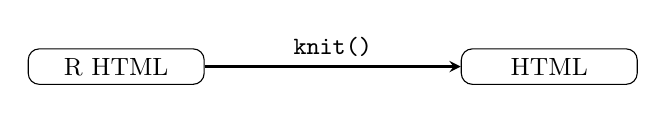
\begin{tikzpicture}[node distance=3cm]
    \node(in)[simple, fill=white, text width=2cm]{R HTML};
    \node(out)[simple, fill=white, text width=2cm, right of=in, xshift=2.5cm]{HTML};
    \draw[arrow](in)--node[anchor=south]{\small{\texttt{knit()}}} (out);
  \end{tikzpicture}
\end{figure}

\section{Introduction}
\label{sec:3.1}
The primary objective of the initial phase is to design and achieve a complete reproducible, invertible workflow. There are many obstacles that limit the possibility of devising an invertible workflow. A sizable one of these problems is that converting (or inverting) between two different document formats requires a tremendous amount of a particular resource that we were limited on; \emph{time}.

Out of the many formats that \textbf{knitr} supports, R HTML is the format we have chosen for the objective. There are two main reasons for this choice; R HTML does not require conversion between two document formats and it allows the use of powerful text processing tools, all of which increase our chance of accomplishing a reproducible, invertible workflow.

%-------------------------------------------------------------------------------
\subsubsection*{Support of unified format}
In \textbf{knitr}, R HTML-based documents are \emph{knitted} to produce HTML-based documents. The \emph{only} difference between these two document formats is that R HTML-based documents contain sections of lines of R code, known as R Code Chunks. Here is an example of a simple R Code Chunk:
\begin{lstlisting}[numbers=none, frame=none]
<!--begin.rcode
plot(cars)
end.rcode-->
\end{lstlisting}
By using the function, \texttt{knit()}, in \textbf{knitr}, the R Code Chunk is run in R to produce output (a plot for the previous example). The R code, \texttt{plot(cars)}, and the output plot are, then, enclosed separately in nested \texttt{div} elements in the final HTML-based document.

\textbf{Knitr} generates HTML documents, as output, from \emph{HTML-based} R HTML documents, as input. In other words, the document generation process does not involve conversion between two distinct document formats. The source document format is essentially the same as the final document format.

By this property, difficulties associated with inverting a document format back into a different format can be minimised and the chance of inverting is increased.

%-------------------------------------------------------------------------------
\subsubsection*{Availability of tool sets}
HTML is markup language very similar to XML. This means powerful XML-based tool sets, such as XPath (REF), are available for use to manipulate the HTML documents effectively. The R package, \textbf{XML} (REF), is used to provide these XML-based tool sets in R.

%-------------------------------------------------------------------------------
\subsubsection*{Demonstration}
Here is a brief demonstration of how an R HTML document can be used to generate a HTML document.

Listing \ref{lst:2.1} is the code structure of the source document, \texttt{example1.Rhtml}. The highlighted text (lines 8--10) is an R Code Chunk. The option, \texttt{echo=FALSE}, is used to hide the R code in the final document.
\definecolor{c}{HTML}{CCFF00}
\newcommand{\hl}[3][black]{{\fboxsep0.5pt\colorbox{#2}{\color{#1} #3}}}
\begin{lstlisting}[caption={\texttt{example1.Rhtml}}, escapechar=\|, label={lst:2.1}]
<!DOCTYPE html>
<html>
<head>
</head>
  <body>
    <h1>Example</h1>
    <p>Summary of the cars data:</p>
    |\hl{c}{<!--begin.rcode echo=FALSE}|
    |\hl{c}{summary(cars)}|
    |\hl{c}{end.rcode-->}|
  </body>
</html>
\end{lstlisting}

The following R code is used to \emph{knit} the source document, \texttt{example1.Rhtml}, to generate the final document, \texttt{example1.html}:
\begin{lstlisting}[numbers=none, frame=none]
> library(knitr)
> knit("example1.Rhtml")
\end{lstlisting}

Listing \ref{lst:2.2} shows the code structure of the final document, \texttt{example1.html}. The R code from line 9 of Listing \ref{lst:2.1} is run in R to produce the result seen in lines 13--19 of Listing \ref{lst:2.2}. Cautions must be taken as the code in Listing \ref{lst:2.2} has been tidied up with line endings to enhance readability. The actual untidied code consists of long lines that usually require text-wrap to fit into the page.
\begin{lstlisting}[caption={(tidied) \texttt{example1.html}}, escapechar=\|, label={lst:2.2}]
<!DOCTYPE html>
<html>
<head>
  <style type="text/css"> ... </style>
</head>
  <body>
    <h1>Example</h1>
    <p>Summary of the cars data:</p>
    <div class="chunk" id="unnamed-chunk-1">
      <div class="rcode">
      <div class="output">
        <pre class="knitr r">
          ##      speed           dist    
          ##  Min.   : 4.0   Min.   :  2  
          ##  1st Qu.:12.0   1st Qu.: 26  
          ##  Median :15.0   Median : 36  
          ##  Mean   :15.4   Mean   : 43  
          ##  3rd Qu.:19.0   3rd Qu.: 56  
          ##  Max.   :25.0   Max.   :120
        </pre></div>
      </div></div>
  </body>
</html>
\end{lstlisting}

Figure \ref{fig:2.1} shows what \texttt{example1.html} will look like in a web browser.
\begin{figure}[h!]
% wkhtmltopdf
\fbox{\includegraphics[trim=0cm 22.5cm 0cm 1cm,clip=true,width=1.1\textwidth,center]{example1}}
\caption{\texttt{example1.html} in a browser}
\label{fig:2.1}
\end{figure}

%------------------------------------------------------------------------------
%--------------------------------- Overview -----------------------------------
%------------------------------------------------------------------------------
\pagebreak
\section{Overview}
\label{sec:overview}

A complete cycle of the invertible workflow consists of six stages. Each stage is involved primarily with text processing, along with an occasional use of XPath.

\begin{figure}[h!]
\centering
  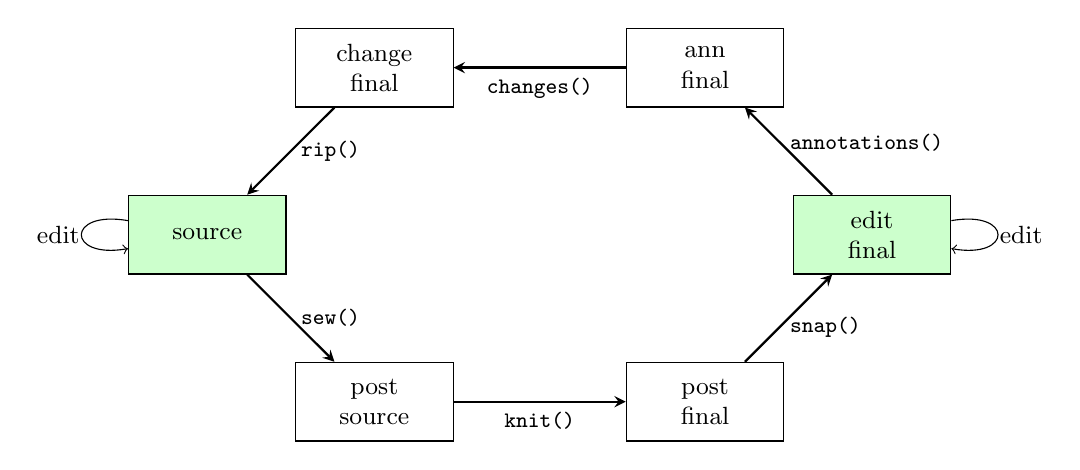
\begin{tikzpicture}
    \node(start)[process, fill=green!20] {source};
    \node(sew)[node distance=3cm, process, below right of=start] {post source};
    \node(knit)[node distance=4.2cm, process, right of=sew] {post final};
    \node(snap)[fill=green!20, node distance=3cm, process, above right of=knit] {edit final};
    %\node(browser)[simple, right of=snap, xshift=2cm]{browser:\\upload, edit, save};
    \node(anno)[node distance=3cm, process, above left of=snap] {ann final};
    \node(chgs)[node distance=4.2cm, process, left of=anno] {change final};
    \draw[arrow](start)--node[anchor=west] {\footnotesize{\texttt{sew()}}} (sew);
    \draw[arrow](sew)--node[anchor=north] {\footnotesize{\texttt{knit()}}} (knit);
    \draw[arrow](knit)--node[anchor=west, pos=0.4] {\footnotesize{\texttt{snap()}}} (snap);
    \draw[arrow](snap)--node[anchor=west, pos=0.6] {\footnotesize{\texttt{annotations()}}} (anno);
    \draw[arrow](anno)--node[anchor=north]{\footnotesize{\texttt{changes()}}} (chgs);
    \draw[arrow](chgs)--node[anchor=west] {\footnotesize{\texttt{rip()}}} (start);
    \draw [->] (start) to [loop left, in=190, out=170, distance=8mm] node[anchor=east, xshift=1mm] {\small{edit}} (start);
    \draw [->] (snap) to [loop right, in=350, out=10, distance=8mm] node[anchor=west, xshift=-1mm] {\small{edit}} (snap);
    %\draw[arrow] (snap) to [out = 30, in = 120, looseness = 1] (browser);
    %\draw[arrow] (snap) to [bend left = 30] (browser);
    %\draw[arrow] (browser) to [bend left = 30] (snap);
    %
    %\draw[line, dashed](rip)-|(repeat);
    %\draw[arrow, dashed](repeat)|-(start);
  \end{tikzpicture}
\caption{The reproducible, invertible workflow}
\label{fig:4}
\end{figure}

%-------------------------------------------------------------------------------
\subsubsection*{Loss of information}
Processing of a source document into a final document can be associated with loss of information from the source document. For example, the original R code in line 9 of Listing \ref{lst:2.1} does not appear in the final document (Listing \ref{lst:2.2}). As a solution, a source document undergoes a pre-processing step where each R Code Chunk is copied in such a way that the original R Code Chunks are perfectly preserved throughout the stages of the workflow and are retainable after a complete cycle.

The pre-processing task is carried out by the function, \texttt{sew()}.

%-------------------------------------------------------------------------------
\subsubsection*{Gain of information}
As opposed to losing information, the document generation process can result in gain of new information. For example, lines 9--19 of Listing \ref{lst:2.2}, which correspond to the output generated from the original R code in line 9 of Listing \ref{lst:2.1}, only exist in the post-processed (final) document. The sections of newly gained information, i.e., the output of R Code Chunks, may seem editable to the client.

However translating changes made on the gained information in the final document to the source document where the new information is non-existent (the output is not generated yet) is problematic. And more technical side of the report, such as manipulating R code, is usually best left for the consultant.

A solution chosen for this project is to restrict these R-created sections of the final document to be annotated only. In this way, the client can still pass on feedbacks to the consultant without directly changing the R code or the output of the R code.

%-------------------------------------------------------------------------------
\subsubsection*{Editing final document}
Allowing the client to modify the final document is achieved by adding JavaScript code to the final document. The JavaScript code loads two libraries, \textbf{CKEditor} (REF) and \textbf{Annotator} (REF), that provide relatively user-friendly GUIs.

The JavaScript code is added by the function, \texttt{snap()}.

\subsubsection*{Merging changes}
Annotations and changes made on the final document are merged by the functions, \texttt{annotations()} and \texttt{changes()}, respectively.

The final stage of the invertible workflow involves text processing to remove any artifacts added by \textbf{knitr} and is carried out by the function, \texttt{rip()}.


%The flow chart in Figure \ref{fig:4} outlines a series of steps involved in our hypothesised round trip. A brief description for each step is as follows:
%\begin{enumerate}[i]
%\item The function \texttt{sew()} is called on the source document (\texttt{.Rhtml}) to generate a \texttt{.post.Rhtml} file.
%
%Each R code chunk in the source document is copied with a slight change to preserve each of the original R code chunks. The goal is to compensate for the fact that the original R code is heavily modified by \textbf{knitr} as the final document is generated (refer back to Listing \ref{lst:2.2} as a reminder). We must preserve the original R code so that it can be ``reproduced" or reappear in the new source document generated from the round trip.
%
%%------------------
%\item The \texttt{.post.Rhtml} document is knitted to produce a \texttt{.post.html} document which retains the copies of the original R code chunks.
%
%Note that these copies are not displayed as they are hidden inside HTML comment tags while the information of the original R code is retained in the subsequent steps. The copies will not be interfered until the very last step of the round trip.
%
%%------------------
%\item The function \texttt{snap()} is called on the \texttt{.post.html} document to produce a \texttt{.edit.html} document.
%
%The main task carried out by \texttt{snap()} is to append a few supplementary lines of code in the \texttt{.post.html} document to enable the features of text editing and annotating. The sections of the document relating to R such as R code chunks and any output from R are restricted for annotations only while the rest of the document is entirely editable with a few possible exceptions (the reason behind this decision will be discussed in more detail later).
%
%Once the output document (\texttt{.edit.html}) is generated (by \texttt{snap()}), it needs to be uploaded onto a server through which editing, annotating and saving the changes made are fully functional. The changes are saved as text files.
%
%%------------------
%\item The saved text file (from the previous step) contains information on any annotations made. The function \texttt{annotations()} can access this information to make appropriate changes on the \texttt{.edit.html} document to produce a \texttt{.anns.html} document.
%
%In the output document (\texttt{.anns.html}), a message is inserted at the top of each annotated R code chunk to display \emph{which} text is annotated with \emph{what} annotations by \emph{who}.
%
%%------------------
%\item Similarly to the previous annotations step, any changes made on the \texttt{.edit.html} document are accessed through the saved text file.
%
%The old, unwanted lines of text from the input document \texttt{.anns.html} are replaced with the corresponding new lines of text to generate a \texttt{.save.html} document.
%
%%------------------
%\item The function \texttt{rip()} is called on the \texttt{.save.html} document to produce a \texttt{.return.Rhtml} document.
%
%The main goal of \texttt{rip()} is to ``reproduce" a new source document with the changes and annotations made the previous steps. It essentially aims to convert the \texttt{.save.html} document to match the format of the source document (\texttt{.Rhtml}). Any additional lines of code inserted during the round trip and the lines added by \textbf{knitr} (such as the lines of code for the style defined by \textbf{knitr}) are removed as the main algorithm for the reproducibility.
%
%\end{enumerate}
%
%Important assumptions and more detailed discussion of these functions involved in the round trip will be introduced in Section %\ref{sec:functions}.

% %------------------------------------------------------------------------------
% % Functions
% %------------------------------------------------------------------------------
% \section{Functions}
% \label{sec:functions}
% There have been various ideas to support the logic behind the algorithms involved in the steps of the round trip. It is absolutely vital to explore deeper into each function for us to gain better understanding. The main purpose of this section is to simply discuss the role of each function in more detail in order to obtain adequate understanding of the overall project and hopefully answer any questions and uncertainties raised in the previous section.
% 
% \subsection{\texttt{sew()}}
% \label{subsec:1}
% One of the most important ideas to constantly remind ourselves was the preservation of the original R code. As briefly mentioned in Section \ref{sec:overview}, retaining the exactly identical R code (that we started with) is a fundamentally important aspect of the round trip in order to reproduce the identical source document. We have figured that the task of preserving the original R code would be much more difficult once the code is converted by the function \texttt{knit()}, as it would then require an extra step of text-processing on the converted R code. Gathering the original information from the converted format is unnecessary complication that we can avoid, which led us to a conclusion that the preservation should happen prior to the conversion step of \texttt{knit()}.
% 
% A possible solution is to formulate a similar strategy that the package \textbf{knitr} uses. As a reminder we can refer back to Listing \ref{lst:1} and note the way R code is presented. The original line of R code is wrapped inside slightly modified HTML comment tags (lines 9 and 11) which act as a marker to signal that the contents in these comments are intended to be displayed in the final document. In other words, the function \texttt{knit()} recognises these specific types of HTML comments and convert their contents (lines of R code) appropriately for display. The package requires the user to enclose all R code chunks intended for display in final documents in this special manner.
% 
% We have decided to implement a similar algorithm involving HTML comment tags through which the retention of the original R code is possible. The only conceptual difference between the two algorithms is in their objectives: detection of R code chunks for conversion in \textbf{knitr} and for preservation in ours. The algorithm we have formulated is to copy the original chunks of R code and insert the copies below the originals. In addition, the HTML comment tags to contain the copies are further modified so that they are explicitly controllable in later steps while avoiding detection from \texttt{knit()}. These copies remain technically as comments in the HTML syntax which can only be examined through the internal code structure of the document (hidden from display through a browser). As a result, the copies of R code chunks (generated by \texttt{sew()}) are preserved in all steps unless we decide to control them to undergo modification.
% 
% In summary, our function \texttt{sew()}:
% \begin{itemize}
%  \item detects any R code chunks that obey the required syntax of \textbf{knitr}, that is the chunks intended to be displayed in final documents, \\[-3ex]
%   \item creates identical copies of those (original) R code chunks with altered the comment tags and \\[-3ex]
%   \item inserts the copies below the corresponding R code chunks.
% \end{itemize}
% 
% The following command in R calls \texttt{sew()} on \texttt{example1.Rhml} to generate \texttt{example1.post.Rhtml}.
% 
% <<eval=FALSE>>=
% source("sew.R")
% sew("example1.Rhtml")
% @
% 
% Listing \ref{lst:3} shows the structure of the output document \texttt{example1.post.Rhtml} from \texttt{sew()}. Note that the code structures of the input document \texttt{example1.Rhtml} (Listing \ref{lst:1}) and the output document \texttt{example1.post.Rhtml} (Listing \ref{lst:3}) are identical except the highlighted text which represents the copy of the original R code (lines 9--11).
% 
% \begin{lstlisting}[caption={\texttt{example1.post.Rhml}}, escapechar=\|, label={lst:3}]
% <!DOCTYPE html>
% <html>
%   <head>
%     <title>Example</title>
%   </head>
%   <body>
%     <h1>Example</h1>
%     <p>20 random variates from the standard normal distribution</p>
%     <!--begin.rcode
%     rnorm(20)
%     end.rcode-->
%     |\hl{c}{<!--begin.keepcode}|
%     |\hl{c}{rnorm(20)}|
%     |\hl{c}{end.keepcode-->}|
%   </body>
% </html>
% \end{lstlisting}
% %------------------------------------------------------------------------------
% \subsubsection{\texttt{knit()}}
% \label{subsubsec:1}
% 
% The output document \texttt{example1.post.Rhtml} from the function \texttt{sew()} is ready to undergo the knitting procedure in a sense that the resultant document \texttt{example1.post.html} (from \texttt{knit()}) will always retain the original R code.
% 
% The following code is executed in R to knit the input document \texttt{example1.post.Rhtml}...
% <<eval=FALSE>>=
% knit("example1.post.Rhtml")
% @
% ...to generate the output document \texttt{example1.post.html} whose internal code structure can be examined in Listing \ref{lst:4}. Note that the highlighted lines represent that the copy of the original R code chunk which remains untouched by the knitting procedure.
% 
% \begin{lstlisting}[caption={\texttt{example1.post.Rhml}}, escapechar=\|, label={lst:4}]
% <!DOCTYPE html>
% <html>
%   <head>
%     |\emph{...lines of style from knitr}|
%     <title>Example</title>
%   </head>
%   <body>
%     <h1>Example</h1>
%     <p>20 random variates from the standard normal distribution</p>
% <div class="chunk" id="unnamed-chunk-1"><div class="rcode"><div class="source"><pre class="knitr r"><span class="hl kwd">rnorm</span><span class="hl std">(</span><span class="hl num">20</span><span class="hl std">)</span>
% </pre></div>
% <div class="output"><pre class="knitr r">##  [1]  0.21997 -1.02766  1.22804  0.78368 -0.09822 -1.41733  0.25276
% ##  [8] -0.89354  0.01876  2.55360 -0.46999  1.14496  0.57621 -0.12584
% ## [15] -0.40660 -1.74065  0.27885  0.90726 -0.97394  0.62497
% </pre></div>
% </div></div>
% 
%     |\hl{c}{<!--begin.keepcode}|
%     |\hl{c}{rnorm(20)}|
%     |\hl{c}{end.rcode-->}|
%   </body>
% </html>
% \end{lstlisting}
% 
% Figure \ref{fig:4} shows how the document \texttt{example1.post.html} looks like in a browser. We should notice that the copy of the origiinal R code is hidden from the display and the only differences in the browser-display are the random variates.
% 
% \begin{figure}[h]
% \includegraphics[trim=0cm 23cm 0cm 0cm,clip=true,width=1.1\textwidth,center]{example1_post}
% \caption{\texttt{example1.post.html} in a browser}
% \label{fig:4}
% \end{figure}
% 
% %------------------------------------------------------------------------------
% \pagebreak
% \subsection{\texttt{snap()}}
% \label{subsec:2}
% So far, we have managed to come up with a way to execute the function \texttt{knit()} on source documents (\texttt{.Rhtml}) while preserving the original information of R code chunks. The next stage of the round trip reflects on our primary objective (of the project), that is to be able to directly edit HTML documents that \texttt{knit()} produces. Possible complications involving the restriction due to \textbf{knitr}'s unidirectional document generation (Section \ref{ch:motiv}) have led us to a decision to implement the use of annotations. Especially the sections of R-related contents in final documentation are considered pointless to be directly edited as it will only result in text-based modification and will not have any impact on generating new results from the modified code. To gain the conceptual benefits of editing as discussed in Section \ref{ch:motiv}, these sections of R-associated contents are decided to be annotated to effectively deliver necessary messages from a person (editor) to another (viewer).
% 
% The first task of the function \texttt{snap()} is designed to identify the parts of an input document that should be editable. The editable sections are identified by searching for all top level elements inside the HTML body of the input document that are not introduced by the function \texttt{knit()}. Then two special attributes are inserted into the opening tag of each of these identified, editable elements: one to serve as a marker to let us know the corresponding element is editable and the other to ``number" the editable elements so that we can deal with them in an orderly manner in later steps. The top elements of annotatable sections (the R-associated contents) are identified by their distict attributes defined by \textbf{knitr}.
% After correctly identifying and marking up all the editable elements, the input document is appended with two supplementary sections of code, namely \texttt{button.html} and \texttt{edit.js}. The HTML code piece \texttt{button.html} contains definition of the designs for two HTML buttons called \texttt{save} and \texttt{submit} while the JavaScript code piece \texttt{edit.js} includes a few assigned instructions. Firstly, \texttt{edit.js} loads the \textbf{jQuery} library and two JavaScript modules named \textbf{CKEditor} and \textbf{AnnotateIt} whose respective functions are to enable browser-based editing and annotating on HTML documentation. Secondly, \texttt{edit.js} is instructed with the actions for the \texttt{save} button, which is to save any changes and annotations made via \textbf{CKEditor} and \textbf{AnnotateIt} as separate text files on a server, and for the \texttt{submit} button, which is to re-direct the browser to an uploading web page on the server (which will be discussed shortly) as well as saving the changes and annotations.
% 
% Once the input document is merged with the contents of \texttt{button.html} and \texttt{edit.js}, an \texttt{.edit.html} document is generated as the output of the function \texttt{snap()}. The resulting \texttt{.edit.html} document is then uploaded onto our test server through which the actual editing and annotating of the document occur. If we refer back to Listing \ref{lst:4}, the lines 10, 11 and 12 are the three top level elements inside the body of the HTML document. By our definition, the first two elements (lines 10 and 11), which correspond respectively to a (most important) heading and a paragraph, are editable and the third element (line 12), characterised by the attribute \texttt{class="chunk"} as an element added by \textbf{knitr}, is annotatable.
% 
% The following code is used in R to call the function \texttt{snap()} on the input document \texttt{example1.post.html} to generate the output document \texttt{example1.edit.html}.
% 
% <<eval=FALSE>>=
% source("snap.R")
% snap("example1.post.html")
% @
% 
% Listing \ref{lst:5} exhibits the internal code structure of the output document. The highlighted text (lines 10 and 11) shows the attributes added by the function \texttt{snap()}. Note that the first attributes \texttt{contenteditable="true"} are used to let \texttt{snap()} recognise the corresponding elements as editable and the second \texttt{id="Editor"} attributes are used to mark up the elements in a sequential manner.
% 
% \begin{lstlisting}[caption={\texttt{example1.edit.html}}, escapechar=\|, label={lst:5}]
% <!DOCTYPE html>
% <html>
%   <head>
%     |\emph{...lines of edit.js...}|
%     |\emph{...lines of style from knitr...}|
%     <title>Example</title>
%   </head>
%   <body>
%     |\emph{...lines of button.html...}|
%     <h1 |\hl{c}{contenteditable="true"}| |\hl{c}{id="Editor-1"}|>Example</h1>
%     <p |\hl{c}{contenteditable="true"}| |\hl{c}{id="Editor-2"}|>20 random variates from the standard normal distribution</p>
% <div class="chunk" id="unnamed-chunk-1"><div class="rcode"><div class="source"><pre class="knitr r"><span class="hl kwd">rnorm</span><span class="hl std">(</span><span class="hl num">20</span><span class="hl std">)</span>
% </pre></div>
% <div class="output"><pre class="knitr r">##  [1]  0.21997 -1.02766  1.22804  0.78368 -0.09822 -1.41733  0.25276
% ##  [8] -0.89354  0.01876  2.55360 -0.46999  1.14496  0.57621 -0.12584
% ## [15] -0.40660 -1.74065  0.27885  0.90726 -0.97394  0.62497
% </pre></div>
% </div></div>
% 
%     <!--begin.keepcode
%     rnorm(20)
%     end.keepcode-->
%   </body>
% </html>
% \end{lstlisting}
% 
% The \texttt{.edit.html} document is then uploaded on to the test server. The browser-display of the document, on the server, can be seen in Figure \ref{fig:5} where the top and bottom displays represent the editable and annotatable environments of \textbf{CKEditor} and \textbf{AnnotateIt} respectively. Editing occurs by each element, that is each section (of the element) must be clicked separately to bring up the editable environment. Attaching annotations requires the user to have an account with \textbf{AnnotateIt} and be logged into their website \url{http://annotateit.org/}. In addition, annotations are made on selections of text of the annotatable sections. Notice the \texttt{save} and \texttt{submit} buttons at the top of the display which can be clicked to save the changes and annotations made. It is of great importance to keep in mind that the execution of editing and annotating takes place simultaneously on the uploaded document to create two separate save files with the information on the annotations and the text-based changes when the \texttt{save} or \texttt{submit} button is clicked.
% 
% \begin{figure}[h]
% \includegraphics[trim=0cm 9cm 0cm 3.5cm,clip=true,width=1\textwidth,center]{CKEditor}
% \includegraphics[trim=0cm 11.5cm 0cm 3.5cm,clip=true,width=1\textwidth,center]{AnnotateIt}
% \caption{\texttt{example1.edit.html}, uploaded on the server, in a browser}
% \label{fig:5}
% \end{figure}
% 
% In summary, the function \texttt{snap()}:
% \begin{itemize}
%  \item identifies and marks up all editable top level elements, present in input documents, in a sequential manner, \\[-3ex]
%  \item appends the two supplementary sections of code \texttt{buttons.html} and \texttt{edit.js} into the input documents whose respective purposes are: \\[-3ex]
%  %
%  \begin{enumerate}[i]
%   \item the provision of the designs for the two \texttt{save} and \texttt{submit} buttons and \\[-3ex]
%   \item to load the \textbf{jQuery} library, enable \textbf{CKEditor} and \textbf{AnnotateIt} on editable and annotatable sections of the input documents respectively, and save the changes and annotations made through the two JavaScript modules as text files on the test server when the buttons are clicked, with an additional feature of re-directing the browser to the uploading web page when the \texttt{submit} button is clicked, and
%  \end{enumerate}
%  %
%  \item finally generate \texttt{.edit.html} documents as the output which can then be uploaded onto the server for the actual editing and annotating of the documents to take place.
% \end{itemize}
% 
% %------------------------------------------------------------------------------
% \subsection{\texttt{annotations()}}
% \label{subsec:3}
% The information on annotations made via the JavaScript module \texttt{AnnotateIt} is accessed from the test server as a text file. The module generates the save file in the JSON format for which we have decided to use an R package called \textbf{jsonlite} to effectively deal with the file format. The save file can be directly fetched from the server by using another R package \textbf{RCurl} and can then be processed, in the manner regarding the JSON format, to generate a message for each annotation. The most informative data such as the selection of text for annotations, the author of the annotations and the annotations themselves are extracted from the save file in order to generate the message.
% 
% Figure \ref{fig:6} is a minimal demonstration of creating an annotation. The last random variate is selected to be marked with the annotation ``Example". Upon clicking the blue \texttt{Save} button on the pop-up window, a save file is created by \textbf{AnnotateIt} on the test server.
% 
% \begin{figure}[h]
% \includegraphics[trim=0cm 11.5cm 0cm 3.5cm,clip=true,width=1\textwidth,center]{annotations}
% \caption{annotating on \texttt{example1.edit.html}}
% \label{fig:6}
% \end{figure}
% 
% The following code is used in R to call the function \texttt{annotations()} on the input document \texttt{example1.edit.html} to generate the output document \texttt{example1.anns.html}.
% 
% <<eval=FALSE>>=
% source("annotations.R")
% annotations("example1.edit.html")
% @
% 
% Listing \ref{lst:6} is the internal code structure of the output document \texttt{example1.anns.html} where the highlighted lines of text (lines 12--14) represent the message genereated according to the information from the save file. The message is in a paragraph tag with the \texttt{class="annotation"} and its own style attributes.
% 
% \begin{lstlisting}[caption={\texttt{example1.anns.html}}, escapechar=\|, label={lst:6}]
% <!DOCTYPE html>
% <html>
%   <head>
%     |\emph{...lines of edit.js...}|
%     |\emph{...lines of style from knitr...}|
%     <title>Example</title>
%   </head>
%   <body>
%     |\emph{...lines of button.html}|
%     <h1 contenteditable="true" id="Editor-1">Example</h1>
%     <p contenteditable="true" id="Editor-2">20 random variates from the standard normal distribution</p>
% |\hl{c}{<p class="annotation" style = "background-color:coral">}|
% |\hl{c}{The text "-1.88681" was annotated with the message "Example" by "e.lim0322"}|
% |\hl{c}{</p>}|
% <div class="chunk" id="unnamed-chunk-1"><div class="rcode"><div class="source"><pre class="knitr r"><span class="hl kwd">rnorm</span><span class="hl std">(</span><span class="hl num">20</span><span class="hl std">)</span>
% </pre></div>
% <div class="output"><pre class="knitr r">##  [1] -0.21445 -0.03694  1.15209 -0.75281  0.66412 -1.14614 -0.98223
% ##  [8] -1.10767 -1.91184  2.00111  0.66261 -1.00241 -0.41161 -0.07720
% ## [15] -1.20503 -1.77474 -1.05262 -3.28418  0.76983 -1.88681
% </pre></div>
% </div></div>
% 
%     <!--begin.keepcode
%     rnorm(20)
%     end.keepcode-->
%   </body>
% </html>
% \end{lstlisting}
% 
% Figure \ref{fig:7} shows the document \texttt{example1.anns.html} in a browser. The text highlighted in red is the message.
% 
% \begin{figure}[h]
% \includegraphics[trim=0cm 19.5cm 0cm 3.2cm,clip=true,width=1.1\textwidth,center]{example1_anns}
% \caption{\texttt{example1.anns.html} in a browser}
% \label{fig:7}
% \end{figure}
% 
% %------------------------------------------------------------------------------
% \subsection{\texttt{changes()}}
% \label{subsec:4}
% The primary task assigned to the function \texttt{changes()} is to access the save file for the changes made through \textbf{CKEditor} from the server and replace the old, modified text (in the input document) with the new text (in the save file). This replacement takes place only for the sections that are actually edited.
% 
% Figure \ref{fig:8} illustrates a brief demonstration of how the process of editing is carried out. The first editable section, which is the heading, is left as it is while the second editable section is chosen to be edited. The original line of text ``20 random variates from..." is to be edited with the bold faced text ``20 normal random variates". When the grey \texttt{save} button is clicked, the save file of the change is created on the server which is a simple text file with the code structure as shown in Listing \ref{lst:7}.
% 
% \begin{figure}[h]
% \includegraphics[trim=0cm 12cm 0cm 3.5cm,clip=true,width=1\textwidth,center]{changes}
% \caption{editing \texttt{example1.edit.html}}
% \label{fig:8}
% \end{figure}
% 
% Note the first line in Listing \ref{lst:7}. This line corresponds to the editable element (in \texttt{example1.edit.html}) with an attribute defined as \texttt{Editor-1}, that is the line 10 in Listing \ref{lst:5}, which is the heading. As we can see the heading is ``\texttt{NOT MODIFIED}" to allow the function \texttt{changes()} to ignore this editable section  of the document. On the other hand, the line 4 displays the desired change on the second editable section.
% 
% \begin{lstlisting}[caption={\texttt{changes.txt}}, escapechar=\|, label={lst:7}]
% EDITOR Editor-1 NOT MODIFIED
% 
% EDITOR Editor-2:
% <strong>20 normal random variates</strong>
% \end{lstlisting}
% 
% The following code is used in R to call the function \texttt{changes()} on the input document \texttt{example1.anns.html} to generate the output document \texttt{example1.save.html}.
% 
% <<eval=FALSE>>=
% source("changes.R")
% changes("example1.anns.html")
% @
% 
% The internal code structure of the output document \texttt{example1.save.html} can be seen in Listing \ref{lst:8}. The highlighted text (line 12) shows that the old line (line 11 in Listing \ref{lst:6}) is replaced with the change (line 4 in Listing \ref{lst:7}) by \texttt{snap()} to result in a display through a browser as shown in Figure \ref{fig:9}.
% 
% \begin{lstlisting}[caption={\texttt{example1.save.html}}, escapechar=\|, label={lst:8}]
% <!DOCTYPE html>
% <html>
%   <head>
%     |\emph{...lines of edit.js...}|
%     |\emph{...lines of style from knitr...}|
%     <title>Example</title>
%   </head>
%   <body>
%     |\emph{...lines of button.html}|
%     <h1 contenteditable="true" id="Editor-1">Example</h1>
%     <p contenteditable="true" id="Editor-2">
% |\hl{c}{<strong>20 normal random variates</strong>}|
%     </p>
%     <p class="annotation" style = "background-color:coral">
%     The text "-1.88681" was annotated with the message "Example" by "e.lim0322"
%     </p>
% <div class="chunk" id="unnamed-chunk-1"><div class="rcode"><div class="source"><pre class="knitr r"><span class="hl kwd">rnorm</span><span class="hl std">(</span><span class="hl num">20</span><span class="hl std">)</span>
% </pre></div>
% <div class="output"><pre class="knitr r">##  [1] -0.21445 -0.03694  1.15209 -0.75281  0.66412 -1.14614 -0.98223
% ##  [8] -1.10767 -1.91184  2.00111  0.66261 -1.00241 -0.41161 -0.07720
% ## [15] -1.20503 -1.77474 -1.05262 -3.28418  0.76983 -1.88681
% </pre></div>
% </div></div>
% 
%     <!--begin.keepcode
%     rnorm(20)
%     end.keepcode-->
%   </body>
% </html>
% \end{lstlisting}
% 
% The text is successfully edited in Figure \ref{fig:9}.
% 
% \begin{figure}[h]
% \includegraphics[trim=0cm 19.5cm 0cm 3.2cm,clip=true,width=1.1\textwidth,center]{example1_save}
% \caption{\texttt{example1.save.html} in a browser}
% \label{fig:9}
% \end{figure}
% 
% %------------------------------------------------------------------------------
% \subsection{\texttt{rip()}}
% \label{subsec:5}
% The main purpose of the function \texttt{rip()} is to return to the original source document format while retaining changes and annotations. It searches for any foreign lines of code that are introduced by \textbf{knitr} or inserted during certain stages of the round trip, and removes those lines. Typically, the lines of the CSS style inserted by \textbf{knitr} are removed first, followed by the lines corresponding to the \texttt{div} elements generated and inserted by \textbf{knitr} (e.g. lines 17--23 in Listing \ref{lst:8}). These \texttt{div} elements are defined with the attribute \texttt{class="chunk"} which can be identified by \texttt{snap()} to recognise them as the elements introduced by \textbf{knitr}. Then the copies of the original R code chunks (lines 12--14 in Listing \ref{lst:3}) are modified by \texttt{snap()} to be exactly as the originals. The text ``\texttt{keep}" in the comment tags of the copy (lines 12 and 14 in Listing \ref{lst:3}) are identified and converted to the letter ``\texttt{r}" so that both the opening and closing comment tags are like the originals. The lines of \texttt{button.html} and \texttt{edit.js} are also removed as well as the two attributes \texttt{contenteditable="true"} and \texttt{id="Editor"}, added to mark up the corresponding elements as editable (Section \ref{subsec:2}).
% 
% The following R code calls the function \texttt{rip()} on the input document \texttt{example1.save.html} to generate the output document \texttt{example1.return.Rhtml}.
% 
% <<eval=FALSE>>=
% source("rip.R")
% rip("example1.save.html")
% @
% 
% The internal code structure of the output document \texttt{example1.return.Rhtml} can be seen in Listing \ref{lst:9}. If we compare the code structure of the source document \texttt{example1.Rhtml} with that of \texttt{example1.return.Rhtml}, we can notice that line 8 in Listing \ref{lst:1} (original) is replaced by the edited text in line 9 of Listing \ref{lst:9}. Lines 11--13 in Listing \ref{lst:9} are the generated messages for the annotations from the previous step (Section \ref{subsec:3}). Apart from these lines, the rest of both documents are identical.
% 
% \begin{lstlisting}[caption={\texttt{example1.save.html}}, escapechar=\|, label={lst:9}]
% <!DOCTYPE html>
% <html>
%   <head>
%     <title>Example</title>
%   </head>
%   <body>
%     <h1>Example</h1>
%     <p>
% <strong>20 normal random variates</strong>
%     </p>
%     <p class="annotation" style = "background-color:coral">
%     The text "-1.88681" was annotated with the message "Example" by "e.lim0322"
%     </p>
%     <!--begin.rcode
%     rnorm(20)
%     end.keepcode-->
%   </body>
% </html>
% \end{lstlisting}
% 
% We can knit the ``final" source document \texttt{example1.return.Rhtml} by the following code in R.
% 
% <<eval=FALSE>>=
% knit("example1.return.Rhtml")
% @
% 
% The display of the knitted document \texttt{example1.return.html} through a browser can be seen in Figure \ref{fig:10}.
% 
% \begin{figure}[h]
% \includegraphics[trim=0cm 22cm 0cm 0cm,clip=true,width=1.1\textwidth,center]{example1_return}
% \caption{\texttt{example1.return.html} in a browser}
% \label{fig:10}
% \end{figure}
% 
% 
% 
% LIMITATIONS section


%------------------------------------------------------------------------------
%----------------------------- Phase 2: Markdown ------------------------------
%------------------------------------------------------------------------------
\chapter{Phase 2: R Markdown}
\begin{figure}[h]
\centering
  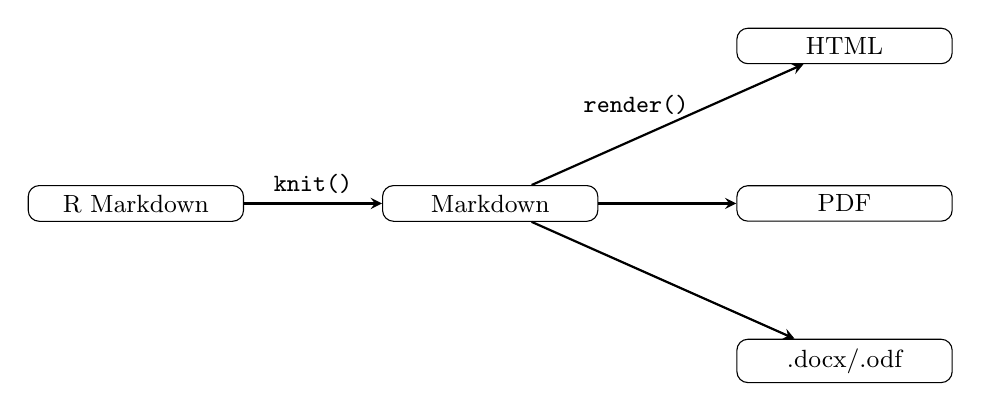
\begin{tikzpicture}
    \node(in)[simple, fill=white, text width=2.5cm]{R Markdown};
    \node(out)[node distance=4.5cm, simple, fill=white, right of=in, text width=2.5cm]{Markdown};
    \node(out1)[node distance=4.5cm, simple, fill=white, right of=out, text width=2.5cm]{PDF};
    \node(out2)[node distance=2cm, simple, fill=white, above of=out1, text width=2.5cm]{HTML};
    \node(out3)[node distance=2cm, simple, fill=white, below of=out1, text width=2.5cm]{.docx/.odf};
    
    \draw[arrow](in)--node[anchor=south]{\small{\texttt{knit()}}} (out);
    \draw[arrow](out)--(out1);
    \draw[arrow](out)--node[anchor=south, xshift=-4mm]{\small{\texttt{render()}}} (out2);
    \draw[arrow](out)--(out3);
  \end{tikzpicture}
\end{figure}

\section{Introduction}
Phase 1 workflow is strictly limited to work on R HTML-based documents in conjunction with \textbf{knitr}. This limitation comes from the way our initial objective has been defined, that is, achieving the workflow (as described in Section \ref{sec:3.1}). Because of this restriction, we do not know whether the workflow is \emph{good} enough or viable elsewhere. It performs exactly as we have designed it to, but is it applicable to other formats?

An important aspect of the workflow to note is the \emph{genericity}. A generic function means that it has specific methods for different types of objects, thus making it very robust. To write a generic piece of code, object-oriented programming is usually considered.

Object-oriented programming (REF) is one of the many programming paradigms that define the fundamental styles of computer programming. R language supports object-oriented programming very well through an \emph{interactive} approach, as opposed to other programming languages, such as C and Java. In this style of programming, an \emph{object} is created by a constructor function and is passed onto \emph{methods} that carry out specific tasks for different types of objects. This means that an object-oriented software is more \emph{generic} to handle different kinds of input more robustly than others.

Unfortunately, the functions invovled in the workflow are neither generic nor object-oriented. As a result, the functions can only handle R HTML- and HTML-based documents as input and phase 1 workflow is strictly limited to work on these two types of document formats. Generalising the workflow or making it object-oriented introduces two problems; the entire workflow may be subject to change, and there is uncertainty to determine if the workflow is worth going through the change.

Let us look at the problems in more detail. Since phase 1 workflow does not involve object-oriented programming, making it to be object-oriented means the entire workflow may require adjustments. Pursuing this will result in a completely different workflow that deviates from the original design we had in mind. In addition, there is no way to determine whether changing the workflow for the sole purpose of making it generic is truly beneficial. Before \emph{any} attempts can be made to improve the workflow, it must be tested, at least, for its applicability. From this test, we can get a rough measure of its potential that may help decide whether to implement changes to the workflow.

In consideration of these problems, the next phase of the project has been decided to explore the applicability of the workflow. The format we have chosen for the second phase is R Markdown. There are four reasons behind our choice; flexibility of R Markdown, easy conversion to HTML, popularity and support.

%-------------------------------------------------------------------------------
\subsubsection*{Flexibility}
R Markdown-based documents are \emph{knitted} to be converted into Markdown (REF), which, in turn, can be converted into different document formats by document conversion software. Depending on the kind of the document converter, PDF, HTML and various other widely used document formats can be generated from Markdown. This flexibility provides the client with options to choose a document format that he or she feels comfortable using.

The document converter we have chosen is \textbf{Pandoc} (REF). \textbf{(Should I write the reasons for this choice?)}

%-------------------------------------------------------------------------------
\subsubsection*{Conversion to HTML}
R Markdown-based documents can be naturally converted into HTML-based documents. This means that once a R Markdown-based source document is processed into a HTML-based final document, phase 1 workflow has a very high chance of being applicable without requiring much adjustment.

%-------------------------------------------------------------------------------
\subsubsection*{Popularity}
Because R Markdown supports flexible conversion, it is increasingly popular and widely used. It has strong emphasis on readability from being an easy-to-read and -write plain text format. This simplicity further increases R Markdown's popularity to be a good candidate for our experiment.

%-------------------------------------------------------------------------------
\subsubsection*{Support for R Markdown}
The latest version, R Markdown v2, has many improvements, one of which, for example, is the support for interactive document generation using \textbf{Shiny} (REF). This is a particularly useful feature in regards to the current global trend.

With the vast advancement in technology, the world demands evidence, often through means of visualising, before acceptance and acknowledgement. In the field of statistics, a particularly effective solution to this demand is via data visualisation, whose effectiveness can be exponentially enhanced by \emph{interactivity}. An interactive visualisation method provides fun and exciting ways to visualise data through which client perception and learning can be greatly improved.

R Markdown's support for \textbf{Shiny}, as well as other improvements, is something that is very promising in securing its already popular usage. It also suggests that R Markdown is relatively active and responsive to meet global demands, thus giving us a reason to choose this document format for phase 2.

%-------------------------------------------------------------------------------
\subsubsection*{Demonstration}
Listing \ref{lst:3.1} is the internal code structure of a simple R Markdown document, \texttt{example2.Rmd}. The highlighted text, lines 6--8, is a simple R Code Chunk.

\begin{lstlisting}[caption={\texttt{example2.Rmd}}, escapechar=\|, label={lst:3.1}]
Example
=========================

Summary of the cars data:

|\hl{c}{```\{r\}}|
|\hl{c}{summary(cars)}|
|\hl{c}{```}|
\end{lstlisting}

There is a crucial difference between the two document generation processes of R HTML and R Markdown. R HTML-based documents are knitted \emph{directly} into HTML, whereas R Markdown-based documents are knitted \emph{intermediately} into Markdown, which is then \emph{rendered} into a final format. Because there are \emph{two} stages involved in one complete document generation process for R Markdown, the function \texttt{knit()} has to be used twice; firstly on the source R Markdown document and secondly on the knitted Markdown document. The difference is significant but can be overlooked. \textbf{Knitr} implements the use of the function, \texttt{render()}, in \textbf{rmarkdown} (REF) package which knits and renders in a single command. 

The R code below calls \texttt{render()} to generate the HTML-based final document, \texttt{example2.html}:
\begin{lstlisting}[numbers=none, frame=none]
rmarkdown::render("example2.Rmd", output_format="html_document")
\end{lstlisting}

Listing \ref{lst:3.2} is the code structure of the final document generated from the source document. The original R Code Chunk in lines 6--8 of Listing \ref{lst:3.1} is processed to produce the result seen in lines 15--21 of Listing \ref{lst:3.2}. In general, the HTML document generated from R Markdown has more content, such as \texttt{meta} elements, than the one from R HTML. Note that there are more than one \texttt{meta}, \texttt{script} and \texttt{style} elements inside \texttt{head} but these are limited to one each for readability.

Even though the two final documents seen in Listings \ref{lst:2.2} and \ref{lst:3.2} are both in the HTML format, they are structurally quite different. Markup attributes such as \texttt{class="container-fluid main-container"} in line 10 of Listing \ref{lst:3.2} is different to \texttt{class="chunk"} markup in line 9 of Listing \ref{lst:2.2}.
\begin{lstlisting}[caption={(tidied) \texttt{example2.html}}, escapechar=\|, label={lst:3.2}]
<!DOCTYPE html>
<html>
<head>
  <meta ... />
  <script> ... </script>
  <style> ... </style>
</head>
  <body>
    <style type="text/css"> ... </style>
    <div class="container-fluid main-container">
      <div id="example" class="section level1">
        <h1>Example</h1>
        <p>Summary of the cars data:</p>
        <pre><code>
          ##      speed           dist    
    	  ##  Min.   : 4.0   Min.   :  2  
    	  ##  1st Qu.:12.0   1st Qu.: 26  
    	  ##  Median :15.0   Median : 36  
    	  ##  Mean   :15.4   Mean   : 43  
    	  ##  3rd Qu.:19.0   3rd Qu.: 56  
    	  ##  Max.   :25.0   Max.   :120
    	</code></pre>
      </div>
    </div>
    <script> ...bootstrap table styles... </script>
    <script> ... mathjax ... </script>    
  </body>
</html>
\end{lstlisting}

Figure \ref{fig:3.1} shows what \texttt{example2.html} will look like in a web browser. Although nearly identical, we can see minor differences between the two final documents, seen in Figures \ref{fig:2.1} and \ref{fig:3.1}, such as different font styles for the headings and spacing used for the R Code Chunk output. The differences are due to different \texttt{styles} used in both cases.
\begin{figure}[h!]
% wkhtmltopdf
\fbox{\includegraphics[trim=0cm 22cm 0cm 1cm,clip=true,width=1.1\textwidth,center]{example2}}
\caption{\texttt{example2.html} in a browser}
\label{fig:3.1}
\end{figure}



%------------------------------------------------------------------------------
%--------------------------------- Overview -----------------------------------
%------------------------------------------------------------------------------
\pagebreak
\section{Overview}
Three additional steps are introduced to phase 2 workflow as a pre-processing stage. Once the source document is \emph{readied} by the three steps of pre-processing, it becomes reproducible and invertible.

Some of the function names kept identical to those in phase 1 workflow to minimise confusion and maintain simplicity. But it must be noted that there are extra features in these functions that work \emph{exclusively} on R Markdown format.

\begin{figure}[h!]
\centering
  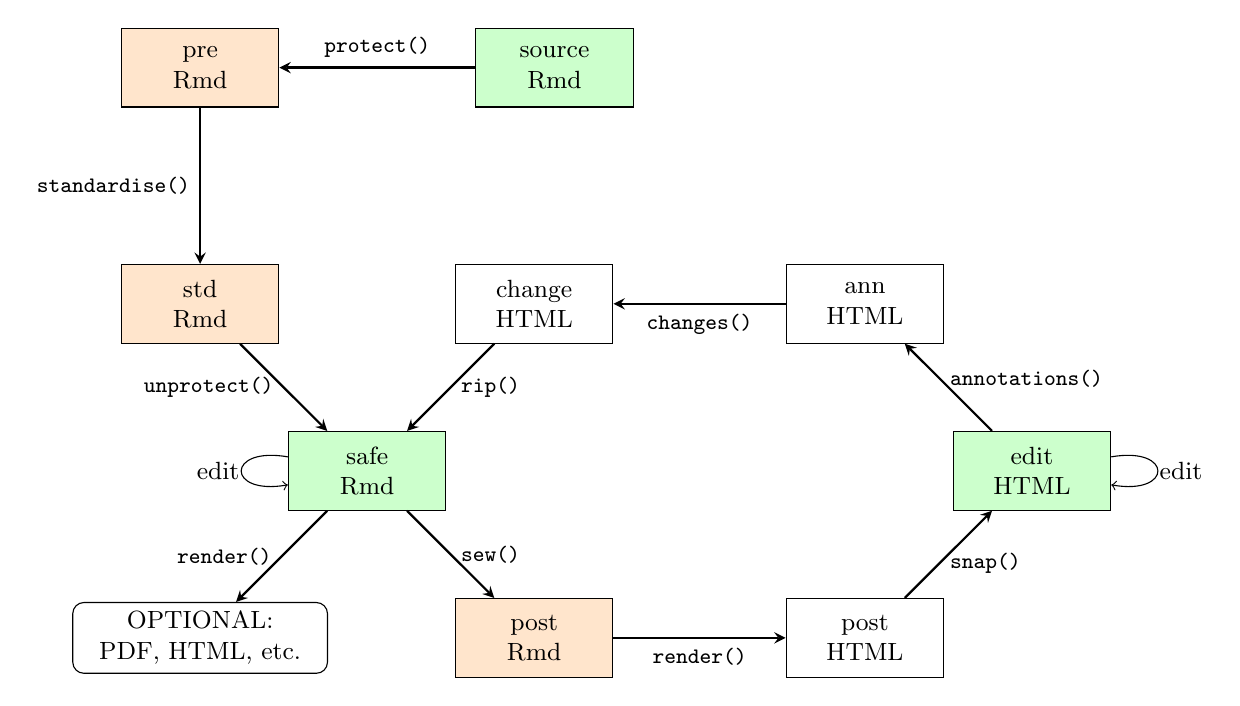
\begin{tikzpicture}
    \node(source)[process, fill=green!20] {source Rmd};
    \node(protect)[node distance=4.5cm, process, fill=orange!20, left of=source] {pre Rmd};
    \node(standardise)[node distance=3cm, process, fill=orange!20, below of=protect] {std Rmd};
    \node(start)[node distance=3cm, process, fill=green!20, below right of=standardise] {safe Rmd};
    \node(sew)[node distance=3cm, process, fill=orange!20, below right of=start] {post Rmd};
    \node(knit)[node distance=4.2cm, process, right of=sew] {post HTML};
    \node(snap)[fill=green!20, node distance=3cm, process, above right of=knit] {edit HTML};
    \node(anno)[node distance=3cm, process, above left of=snap] {ann HTML};
    \node(chgs)[node distance=4.2cm, process, left of=anno] {change HTML};
    %
    \node(output)[simple, node distance=3cm, below left of=start, fill=none] {OPTIONAL: PDF, HTML, etc.};
    \draw[arrow](start) --node[anchor=east] {\footnotesize{\texttt{render()}}} (output);
    %
    \draw[arrow](source) --node[anchor=south] {\footnotesize{\texttt{protect()}}} (protect);
    \draw[arrow](protect) --node[anchor=east] {\footnotesize{\texttt{standardise()}}} (standardise);
    \draw[arrow](standardise) --node[anchor=east] {\footnotesize{\texttt{unprotect()}}} (start);
    \draw[arrow](start)--node[anchor=west] {\footnotesize{\texttt{sew()}}} (sew);
    \draw[arrow](sew)--node[anchor=north] {\footnotesize{\texttt{render()}}} (knit);
    \draw[arrow](knit)--node[anchor=west, pos=0.4] {\footnotesize{\texttt{snap()}}} (snap);
    \draw[arrow](snap)--node[anchor=west, pos=0.6] {\footnotesize{\texttt{annotations()}}} (anno);
    \draw[arrow](anno)--node[anchor=north]{\footnotesize{\texttt{changes()}}} (chgs);
    \draw[arrow](chgs)--node[anchor=west] {\footnotesize{\texttt{rip()}}} (start);
    \draw [->] (start) to [loop left, in=190, out=170, distance=8mm] node[anchor=east, xshift=1mm] {\small{edit}} (start);
    \draw [->] (snap) to [loop right, in=350, out=10, distance=8mm] node[anchor=west, xshift=-1mm] {\small{edit}} (snap);
  \end{tikzpicture}
\caption{Revised reproducible, invertible workflow}
\label{fig:3.2}
\end{figure}

\subsubsection*{Invertibility of \textbf{Pandoc}}
\textbf{Pandoc} does not support flawless conversion between document formats, that is, the source document format is not the same as the final document format.

There is an internal structure in \textbf{Pandoc} that determines the structure of the output documents. This means that whether the source document obeys the internal structure or not, \textbf{Pandoc} will always produce a final document that obeys the internal structure. This is best understood with a simple diagram:
(\textbf{Fix diagram})
\begin{figure}[h!]
\centering
  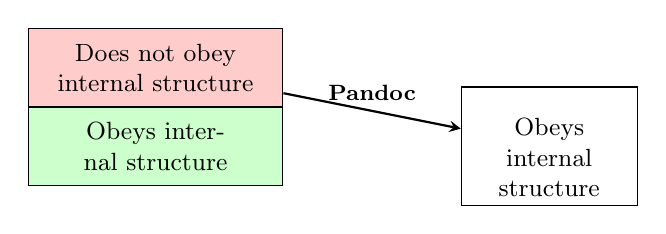
\begin{tikzpicture}[on grid]
    \node (top) {};
    \node(start1)[process, fill=red!20, text width=3cm, right of=top] {Does not obey internal structure};
    \node(start2)[process, fill=green!20, text width=3cm, below of=start1] {Obeys internal structure};
    \node(end1)[node distance=5cm, process, right of=start2, text height=0.5cm, text width=2cm] {Obeys internal structure};
    \draw[arrow](start1)--node[anchor=south] {\footnotesize{\textbf{Pandoc}}} (end1);
  \end{tikzpicture}
\end{figure}

We have decided to use the internal structure as a means of \emph{standardising} the source document so that any subsequent conversion by \textbf{Pandoc} does not interfere with its structure. The structural aspect of standardised documents will be consistent throughout the workflow.

The standardisation step is carried out by the function, \texttt{standardise()} with the use of \textbf{Pandoc}.


%Initially, \textbf{Pandoc} is tested whether it supports perfect, flawless conversion between two document formats, that is, the source document must be identical to the final converted document.
%
%Intuitively, we can use \textbf{Pandoc} on a Markdown-based source document to convert it into HTML, then back to Markdown (e.g., a two-step round trip) and compare the source and final Markdown documents. But these two steps can be further simplified into a single step; the Markdown-based source document can be converted directly to a final \emph{Markdown} document. Hence a simple round trip on a Markdown document is tested for invertibility.
%
%
%Listing \ref{lst:3.3} is the code structure of the source Markdown document, \texttt{example3.Rmd}.
%
%\begin{lstlisting}[caption={\texttt{example3.Rmd}}, escapechar=\|, label={lst:3.3}]
%Header 1
%-------------------------------------------------
%This is an R Markdown document. Markdown is a
%simple formatting syntax for authoring web pages.
%
%Use an asterisk mark, to provide emphasis such as
%*italics* and **bold**.
%
%You can write `in-line` code with a back-tick.
%
%```
%Code blocks display
%with fixed-width font
%```
%
%> Blockquotes are offset
%\end{lstlisting}
%
%The command line below can be run to use \textbf{Pandoc} on the source document to generate the final document, \texttt{exmaple3-pandoc.Rmd}.
%
%\begin{lstlisting}[numbers=none]
%pandoc -t md -f md example3-return.Rmd example3.Rmd
%\end{lstlisting}
%
%Listing \ref{lst:3.4} is the code structure of the final document, \texttt{example3-return.Rmd}. Comparing the source and final documents, we can notice a few differences. Firstly, the number of dashes (line 2 of Listings \ref{lst:3.3} and \ref{lst:3.4}) are different. Secondly, the character width for each line is changed. And finally, the fenced code syntax as seen in lines 11 and 14 of Listing \ref{lst:3.3} disappears and the code block is delimited by tabs (or 4 spaces) in lines 12 and 13 of Listing \ref{lst:3.4}.
%
%\begin{lstlisting}[caption={\texttt{example3-return.Rmd}}, escapechar=\|, label={lst:3.4}]
%Header 1
%--------
%
%This is an R Markdown document. Markdown is a simple formatting syntax
%for authoring web pages.
%
%Use an asterisk mark, to provide emphasis such as *italics* and
%**bold**.
%
%You can write `in-line` code with a back-tick.
%
%    Code blocks display
%    with fixed-width font
%
%> Blockquotes are offset
%\end{lstlisting}
%
%Evidently, \textbf{Pandoc} does not support flawless conversion between document formats and defeats the core concept of invertibility. However, further round trip using the final document, \texttt{example3-return.Rmd}, as the input produces the identical output. This suggests that \textbf{Pandoc} has an internal document structure, that is a set of rules on which the structure of newly generate documents is based.
%
%The internal structure identified so far is that \textbf{Pandoc} matches the length of equal signs and dashes that are used to \emph{underline} headers to the character width of the headers, breaks normal text lines and fenced code regions become delimited with tabs.

%-------------------------------------------------------------------------------
\subsubsection*{Loss of information}
R Markdown has syntax for specifying metadata, such as author, title and date information. An example of a metadata section is as below:
\begin{lstlisting}[numbers=none, frame=none]
---
title: "Example"
output:
  html_document:
    toc: true
    theme: united
---
\end{lstlisting}

Metadata sections are \emph{exclusive} to R Markdown. As a result, \textbf{Pandoc} discards them in its output documents. This means that the metadata information cannot be carried over to subsequent steps after the standardisation step.


%Because \textbf{Pandoc} does not support R Markdown, R Code Chunks are not processed by \textbf{Pandoc} properly. As a result, R Code Chunks are changed with no apparent patterns. For example, the R Code Chunk in lines 6--8 of Listing \ref{lst:3.1} is changed like below:
%
%\begin{lstlisting}[numbers=none]
%`{r, echo=FALSE} summary(cars)
%\end{lstlisting}
%
%The change does not provide a pattern on which reliable text processing can be based. So R Code Chunks are \emph{protected} by enclosing them with special delimiters.
%
%R Markdown format provides metadata sections in which title, author, date and options for customising output can be explicitly specified. This is a feature exclusive to R Markdown, which means metadata sections also require protections against \textbf{Pandoc}.
%
%The function, \texttt{protect()}, protects R Code Chunks and metadata sections. To satisfy invertibility, standardised documents are \emph{unprotected} by the function, \texttt{unprotect()}, that is, any text-based changes from \texttt{protect()} are reverted.

%-------------------------------------------------------------------------------
\subsubsection*{Conversion of formats}


%-------------------------------------------------------------------------------
%------------------------------ Function details -------------------------------
%-------------------------------------------------------------------------------
%\section{Function details}
%\subsection{\texttt{protect()}}
%An \textbf{R Markdown} document typically has a metadata section that contains information for title, author, date and options for customising output (such as theme and table of content availability). The metadata section is \emph{exclusive} to the \textbf{R Markdown} format which means \textbf{Pandoc} does not recognise it as the regular Markdown syntax. As a result, this information is discarded after document conversion process by \textbf{Pandoc} takes place.
%
%When \textbf{Pandoc} converts an \textbf{R Markdown} document into other document types, the R Code Chunks in the document are changed. R Code Chunks are specified by the native Markdown syntax for fenced code regions, thus one might expect them to be regarded as verbatim programming code throughout different document types. However R Code Chunks are modified with no clear patterns to the extent that no reliable text processing could be devised in order to fix the change.
%
%Therefore metadata sections and R Code Chunks are protected, prior to the standardisation by \textbf{Pandoc}. Metadata sections are protected by enclosing them with \texttt{<!--rmd\_metadata} and \texttt{rmd\_metadata--> rmd-rmLines} delimiters, instead of their usual \texttt{---} delimiters. The delimiters used to wrap metadata sections are in the form of a comment in the HTML syntax as they are not interfered by \textbf{Pandoc} and perfectly retainable after standardisation. The text, \texttt{rmd-rmLines}, is used to account for the fact that \textbf{Pandoc} tends to remove empty lines between the end of R Code Chunks and text.
%
%R Code Chunks are protected similarly by delimiting them with \texttt{<!--begin.keepcode} and \texttt{end.keepcode-->} markup. One difference here is that the delimiters are added in front and end of the usual \texttt{```{r}} and \texttt{```} delimiters of R Code Chunks to wrap the entirety of R Code Chunks. This allows for more reliable retention of the R code after standardising, as well as easier text processing.
%
%The output of \texttt{protect()} is in \texttt{.pre.Rmd} format.
%
%
%\subsection{\texttt{standardise()}}
%\textbf{Pandoc} has an internally defined format that its output documents are based on. The internal format of \textbf{Pandoc} for a Markdown document requires that the length of text for header must be equivalent to the length of equal signs or dashes that \emph{underline} the headers in setext-style, and code blocks must be delimited with tabs (or 4 spaces) instead of three backtick quotes.
% 
%When the inversion process by \textbf{Pandoc} is executed on a Markdown document that disobeys the internal format, the inverted document will always be different to the source document
%
%As a result, the number of equal signs and dashes are shortened or extended to match the character width of the text for corresponding headers. Atx-style headers for first two header levels are converted to the setext-style header with the similar length matching, while the other four header levels remain the same. 
%
%Once a protected document is prepared, it is standardised into a format that remains consistent over repeated document conversion by \textbf{Pandoc}. By using the option, \texttt{--no-wrap}, \textbf{Pandoc} does not implement text-wrap, based on its internally defined rule.
%
%
%\subsection{\texttt{unprotect()}}



% %------------------------------------------------------------------------------
% \section{Discussion}
% \label{sec:discussion}
% There are a few restrictions in the round trip that need to be discussed. Some of the steps involved in the round trip base their algorithms on the assumption that \textbf{knitr} remains consistent. For example, identifying the annotatable elements (Section \ref{subsec:2}) is carried out under the assumption that these elements are always given the attribute \texttt{class="chunk"} by \textbf{knitr}. If there is to be a change in \textbf{knitr} that affects the structure of the annotatable elements, especially their attributes, the round trip will fail to complete the cycle and we will have to devise a new measure for the change.
% 
% The editing and annotating stage of the round trip is limited to what \textbf{CKEditor} and \textbf{AnnotateIT} offer as the necessary tools. The requirement by \textbf{AnnotateIT} for its user to maintain a logged-in status with their website is a restriction that can be avoided altogether by implementing a different annotator module. The overall process of editing and annotating can be more efficient and flexible to allow for more extensive document editing by the use of modules that have relatively less restrictions than \textbf{CKEditor} and \textbf{AnnotateIT}.
% 
% Furthermore the efficiency of the round trip may improve by the use of a different HTML editor. One of the main reasons behind the uploading procedure is to enable \textbf{CKEditor} without having to localise the module in the user's computing environment. If it is possible to integrate an HTML editor, into the round trip, that does not pose the localisation problem the uploading step can be omitted to make more efficient and tidier document generation and editing through the round trip possible.
% 
% By using a different HTML editor, we can also reduce some of the problems arising from the uploading stage of the round trip. Currently it is not possible to upload external files such as image files that are produced by R on the test server. As a result, any graphics included in the uploaded documents cannot be displayed through a browser. Again this issue can be avoided by using suitable HTML editors that do not require the server integration. A possible future direction of the project in regards to these limitations is in generalising the round trip so that the user gets to choose which HTML editors to use for the round trip.
% 
% There is a possibility of an alternative approach to the round trip. This would be to integrate a wiki or an online document system (e.g. Google Docs) as the main editing tool. These tools may improve the efficiency of the overall editing process through more dynamic and responsive process of document editing.
% 
% Finally, we need to consider how the sections of images, mathematical equations and general tables could be edited in a document. A possible approach to the problem is to allow annotations on them as we cannot directly interfere with the contents of these sections. A better approach would be to utilise a suitable JavaScript module written for the purpose of editing or annotating on these specific sections.
% 
% %------------------------------------------------------------------------------
% \section{Conclusion}
% Our ultimate goal remains to be in further generalising the round trip to suit a broader spectrum of document types. The first phase of the project has explored the possibilities of a complete round trip between the source and final documents to enhance the flow of the document generation process. So far the phase 1 round trip is strictly limited to the HTML type of documentation. However, we hope that our suggested ideas involved with each step of the round trip can be used by others to further optimise the procedures invovled in statistical document generation.
% 
% %------------------------------------------------------------------------------
% \section{Contributions}
% List of contributions from the project supervisor Dr Paul Murrell:
% \begin{itemize}
%  \item ideas
%  \item \texttt{edit.js}
%  \item \texttt{button.html}
% \end{itemize}

\end{document}

